\section{Spørgsmål 1 - Innovation og Produktudvikling}
Denne opgave har til formål at belyse innovation, produktudvikling, og produktudviklingsstrategi.\\
Dette gøres med afsæt i opgivet pensum samt tre af de artikler opgivet i eksamensopgaven, som vil blive
referet til på følgende måde:\vspace{0.25cm}
\begin{itemize}
    \item \cite[a.1]{eksamensopgave} - "Sådan undgår en virksomhed at forhaste sig på det teknologiske felt"
    \item \cite[a.2]{eksamensopgave} - "Fadøl er det nye våben i et globalt slagsmål"
    \item \cite[a.3]{eksamensopgave} - "Giganterne har rettet sigtekornet mod danske iværksættere"
\end{itemize}
\paragraph{Innovation} er den proces, hvorved organisationer anvender deres ekspertise og
ressourcer til at udvikle nye produkter, for bedre at kunne tilpasse de skiftende
behov der måtte være for forbrugerne på det pågældende marked, eller optimere eksisterende metoder for eksisterende produkter.\\
Innovation bliver ofte brugt som et buzzword for signalere nytænkning, men faktum er, at innovation ofte er en ressourcetung proces og op mod 88\% af projekter ikke når ud til brugerne\cite[s. 388]{jones:2013}.
\subsection{Innovationstyper}
Innovation kan opdeles i to typer, "Incremental Technological Change" og "Quantum Technological Change".
\paragraph{Incremental Technological Change (ITC)} er teknologi som gradvist bliver forfinet eller udbygget baseret på en allerede
eksisterende teknologi, hvor dette er den mest gængse type af innovation, og ses i vid udstrækning, f.eks. hver gang der lanceres en ny model af en allerede eksisterende smartphone\\
Et eksempel på ITC er at finde i artiklen omkring Plant Jammer \cite[a.3]{eksamensopgave}, hvor Miele
har indkøbt sig i virksomheden, antageligt mod at få et økonomisk afkast eller, måske nok mere sandsynligt, indkorporere teknologien
i en ny række af køleskabe, for at skabe en konkurrencedygtig linje af "smart fridges", for at bl.a. Samsung, LG, Electrolux \cite{fridgemarketshare1, fridgemarketshare2}
\\\paragraph{Quantum Technological Change (QTC)} er de ændringer i teknologien som skaber fundamentale ændringer i enten produkterne, eller måden hvorpå de produceres.
Eksempler på dette er bl.a. udviklingen af den første pc og smartphone, som begge revolutionerede IT-industrien, hvor det i dag er svær at forestille sig en verden
uden disse teknologier. Det kan være svært at spå om på forhånd, hvorvidt en ny teknologi eller tilhørende produktionsmetode, vil have denne revolutionerende effekt, der kan dog, med forbehold,
peges på DraughtMaster fra Carlsberg \cite[a.2]{eksamensopgave}, som et eksempel på dette, dog på en noget mindre skala, end de førnævnte.\\
Grunden til dette er udelukkende pga. den enorme ændring i fustagernes holdbarhed, og derved øger forhandlingsmulighederne for mange restaurationer, som ellers ikke ville
kunne omsætte nok i de givne specialøl, til at opveje omkostningerne.
\subsection{First Mover og Follower}
"First Mover" og "First Follower" er termer for de to hovedaktører ift. udnytte innovation til at stå bedre på markedet.
First Mover er innovatørerne bag produktet, og investerer en stor mængde ressourcer, for at komme først på markedet med et nyt produkt, hvor First Follower udnytter det grundlæggende arbejde fra First Movers til at udvikle deres eget lignede produkt.
\\Som tidligere nævnt er der nævneværdige ressourcer forbundet med innovation, hvilket
også betyder, at timing ift. markedet ofte er alfa og omega, og at det i givne situationer kan betale sig at holde igen, hvilket også belyses i artiklen omkring forhastet innovation \cite[a.1]{eksamensopgave}.
Her påpeges det, at det ofte er first followers som vinder andele på markedet, antageligt fordi de kan udnytte det arbejde som first movers har igangsat og samtidig starte med et produkt, som er tilpasset bedre til det nuværende marked.\\
Derved ikke sagt at det udelukkende er en ulempe at være first mover, da der også er forbundet en række store fordele, såfremt produktet har success. Nedenfor oplistes de fordele og ulemper, som kan være forbundet med dem begge.
\paragraph{First Mover}
\begin{itemize}
    \item Fordele
    \begin{itemize}
        \item Mulighed for at oprette patent på det udviklede produkt.
        \item Der er ingen eksisterende konkurrenter af produkttypen på markedet, så kundernes valgmuligheder er begrænset til deres produkt, hvilket også kan medføre en form for standardisering af produktypen fremadrettet.
        \item Organisationen har mere data og erfaring omkring produktet end eventuelle konkurrenter på det pågældende tidspunkt.
    \end{itemize}
    \item Ulemper
    \begin{itemize}
        \item Innovation er en ressourcetung process, og såfremt der ikke udvikles et færdigt produkt, eller udviklingen af denne er for langsom, så er der et potentielt stort økonomisk tab.
        \item Et nyt produkt er ikke garanteret at følge markedet, hvilket også belyses i \cite[a.1]{eksamensopgave}, så der er også en risiko for at produktet ikke passer til markedet på nuværende tidspunkt.
    \end{itemize}
\end{itemize}
\paragraph{First Follower}
\begin{itemize}
    \item Fordele
    \begin{itemize}
        \item Da first movers allerede har investeret en væsentlig mængde ressourcer på udviklingen, er de økonomiske omkostninger for first followers væsentlig lavere.
        \item Det er muligt at vurdere produktet yderligere inden påbegyndelsen af egen udvikling, hvilket reducerer risikoen for at produktet ikke passer til markedet.
    \end{itemize}
    \item Ulemper
    \begin{itemize}
        \item Der er en risiko for at first movers har oprettet patent eller på anden måde beskyttet deres produktet mod nye indtrængere.
        \item Selvom der ikke er forbundet mange ressourcer med den initielle udvikling, som ved first movers, så kan det være nødvendigt at investere en nævneværdig mængde for at sørge for at produktet kommer på markedet inden det bliver fyldt.
    \end{itemize}
\end{itemize}
\subsection{Behovet for innovation og videreudvikling}
For ikke at mætte forbrugerne med en organisations produkter er det vigtigt at vide hvornår der er behov for innovation.
Med et stigende fokus på bæredygtighed, bliver den nye funktionalitet for innovative produkter holdt mere op deres forgængere,
hvilket resulterer i et mere skeptisk marked på nogle punkter \cite[a.1]{eksamensopgave}. Dvs. at når der lanceres et nyt produkt, skal det kunne retfærdiggøre en udskiftning i større grad end før.
\\~\\Ved at anvende produktslivcycklusmodellen (Figur \ref{livscyklusmodel}), kan man se modenheden af produktet og deraf vurdere hvornår det er tid til innovation.
\\Modellen består af fire faser:
\begin{itemize}
    \item \textbf{Udvikling/Introduktion}\\Udviklingen er helt stringent ikke en del af de fire faser, dog illustrer det hvor stor en omkostning der kan være forbundet med innovation, hvorfor den er medtaget her.
    \\Introduktionen er startfasen for produktet på markedet, hvor forbrugerne endnu ikke er begyndt at tage produktet reelt til sig. Og ligesom udviklingen er denne fase omkostningstung, da den primære markedsføring finder sted i denne fase.
    \item \textbf{Vækst}\\I vækstfasen begynder produktet for alvor at fange forbrugernes interesse, og man ser efterspørgslen stige markant ift. introduktionen.
    \item \textbf{Modning}\\Modningsfasen starter når markedet begynder at blive mættet, da de fleste forbrugere har investeret i produktet, og nytilkomne forbrugere bliver færre og færre.
    \\Dette leder til "Replacement Demand" hvor det eksisterende produkt vil kunne blive erstattet, og det er derfor her organisationen skal sætte ind ift. innovation.
    \item \textbf{Nedgang}\\På dette tidspunkt er produktet nærmest døende. Der er meget få nye forbrugere på markedet, og den profit som produktet tidligere har kunne tilbringe organisationen falder stødt.
\end{itemize}
\begin{figure}[H]
    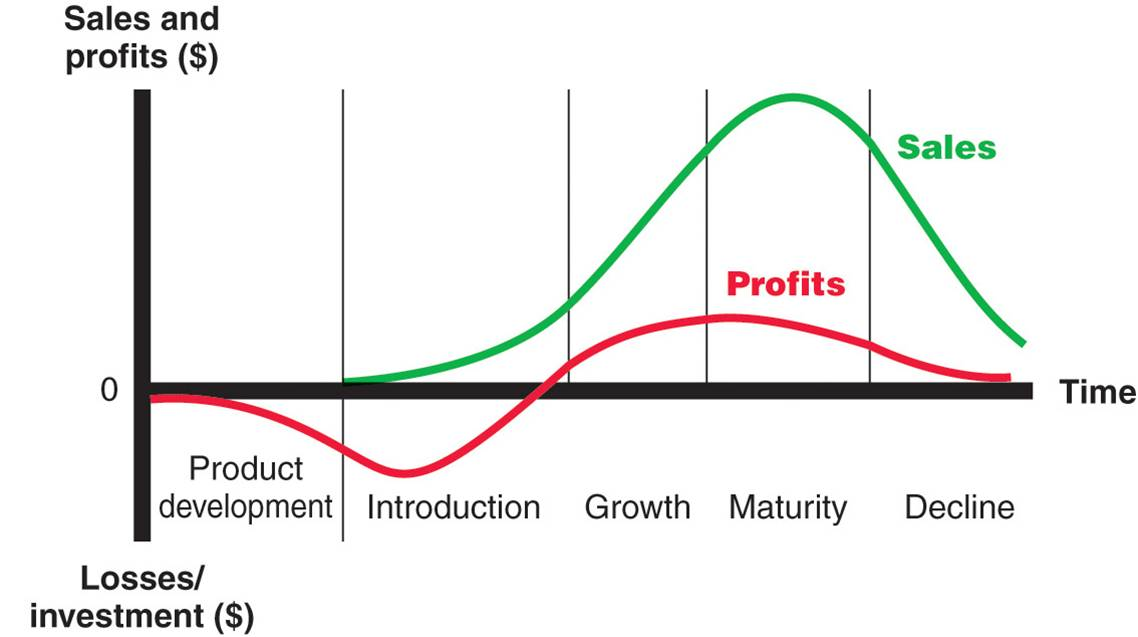
\includegraphics[width=\textwidth]{assets/Product-Life-Cycle-Stages.jpg}
    \caption{produktlivscycklusmodel \cite{plcpic}}
    \label{livscyklusmodel}
\end{figure}
\noindent
Ud fra denne model, er det muligt at estimere behovet for innovation, hvor det optimalt ville finde sted med et modent basisprodukt før den bliver mindre profitabel og forældet,
og forbrugerne søger alternativer ved konkurrenterne, hvor organisationen også samtidig får udnyttet potentialet for økonomisk gevinst.
\\~\\Hvis man holder de to artikler, Carlsberg og Plant Jammer \cite[a.2, a.3]{eksamensopgave}, op mod denne model, ses det at Carlsberg allerede befinder sig i vækstfasen,
antageligt i modsætning til konkurrenterne Heineken og AB Inbev (som pt. ligger i en deadlock pga. en patentkonflikt), da de allerede har leveret systemet til 2500 restaurationer i Danmark, hvilket svarer til over 17\% af de samlede restaurationer i Danmark \cite{restaurantstat}.
\\Plant Jammer befinder sig måske et sted mellem introduktion og vækst, da de allerede har en app tilgængelig. Ifølge Play Store kører de med version 2.48.1 \cite{plantplay}, hvilket giver grund til at antage at de højst sandsynligt har bevæget sig fuldt ind i vækstfasen, da lancering ofter starter ved 1.0, hvor 2.0 er den første markante ekspansion af systemet med yderligere funktionalitet.
\\Dog er det muligt at der vil opstå et form for simultantkørende produkt i forbindelse med deres samarbejde med Miele, hvor de så vil befinde sig i udviklingen med dette.
\subsection{Udviklingsstrategi}
\cite{PDS}Produktudviklingsstrategi er en betegnelse for den proces der bringer ny innovation til forbrugerne.
\\En organisation kan benytte sig af forskellige strategier afhængigt af markedet og organisationens kernekompetencer. Organisationen kan bl.a.
\begin{itemize}
    \item Forbedre eksisterende produkter
    \\Denne strategi er relativ simpel, og består i sin enkelthed i at videreudvikle på eksisterende produkter, for at forblive konkurrencedygtig.
    \item Reducere omkostninger ved produktudvikling
    \\Ved at reducere omkostningnerne forbundet med udvikling af et produkt, kan virksomheden enten tilbyde produktet til en lavere pris, og derved presse konkurrenterne, eller fasthholde prisen og derved gøre produktet mere profitabelt.
    \item Tilknytte værdier til produktet
    \\Som tidligere nævnt fylder den bæredygtige agenda mere for forbrugerne end tidligere \cite[a.1]{eksamensopgave}, hvilket gør det muligt for organisationer at lancere produkter med værdier tilknyttet bæredygtighed.
    Dette er dog blot en af mange værdisæt organisationer kan koble sammen deres produkter. Kosmetikindustrien kobler i stor grad deres produkter sammen med dyrevelfærd, ligeledes gør fødevareindustrien, mens der samtidig er fokus på Fair Trade, for at sikre producenterne af disse bedre vilkår.
    \item Diversificere produktionen
    \\Ved at diversificere produktionen, er det muligt for organisationen at tage deres eksisterende produktlinjer, eller lave nye, og tilpasse det bedre til specifikke grupper af forbrugere. Dette kan være, men er absolut ikke begrænset til grupperinger af køn, alder, kompetencer (eks. indenfor IT eller sport), m.m.
\end{itemize}
\textbf{Stage-Gate Development Funnel}
\\En innovativ organisation lever på ideer, dog er det ikke alle ideer som er lige i et forretningsøjemed. En måde hvorpå disse kan filtreres findes i Stage-Gate Development Funneling.
\begin{figure}[H]
    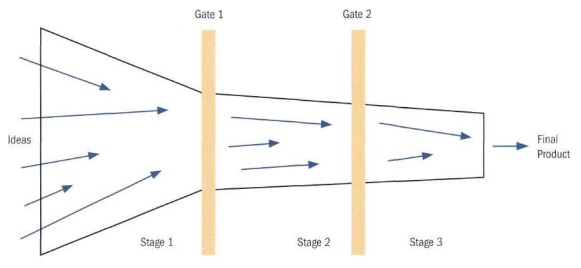
\includegraphics{assets/Stage-Gate.jpg}
    \caption{Stage-Gate Development Funnel \cite[s. 399]{jones:2013}}
    \label{stagegate}
\end{figure}
\noindent Som illustreret i figur \ref{stagegate} tages alle ideerne ifm. produktudvikling og køres igennem forskellige stadier. Modellen er udformet som en tragt, da det initielle input af ideer ønskes at være så stort som muligt for at fremme nytænkning og innovation.
\\De forskellige gates har til formål at fungere som checkpoints, hvorfor det bliver muligt at opsætte nogle krav der kan vurderes efter, for at bestemme om ideen skal gå videre til næste stadie.
\\Det første checkpoint er typisk en vurdering af hvorvidt ideen passer med organisationens kompetencer og mål, samt hvordan produktet ville klare sig på det dertilhørende marked.
\\Ved det andet checkpoint er ideerne blevet uddybet og specificeret, og organisationen vil et panel som vurderer hvorvidt den udvidede ide er værd at udvikle på.
\\~\\En Stage-Gate Funnel består ikke nødvendigvis kun af to gates, og kan tilpasses til de enkelte organisationers preferencer, hvorfor kravene for de forskellige gates også vil være anderledes.
\\~\\Hvis en organisation har for mange ideer, og ikke får disse afgrænset, vil det ofte kunne lede til ufuldendte eller mangelfyldte produkter, hvilket måske kunne have været tilfældet for Carlsbergs DraughtMasteri 2007 \cite[a.2]{eksamensopgave}, hvorfor også Mikkel Flyverbom anbefaler at organisationer at være tro mod dem selv \cite[a.1]{eksamensopgave}.